\documentclass{standalone}
\usepackage{tikz}
\usetikzlibrary{patterns, positioning}
\usepackage[sfdefault]{ClearSans} %% option 'sfdefault' activates Clear Sans as the default text font
\usepackage[T1]{fontenc}

\begin{document}
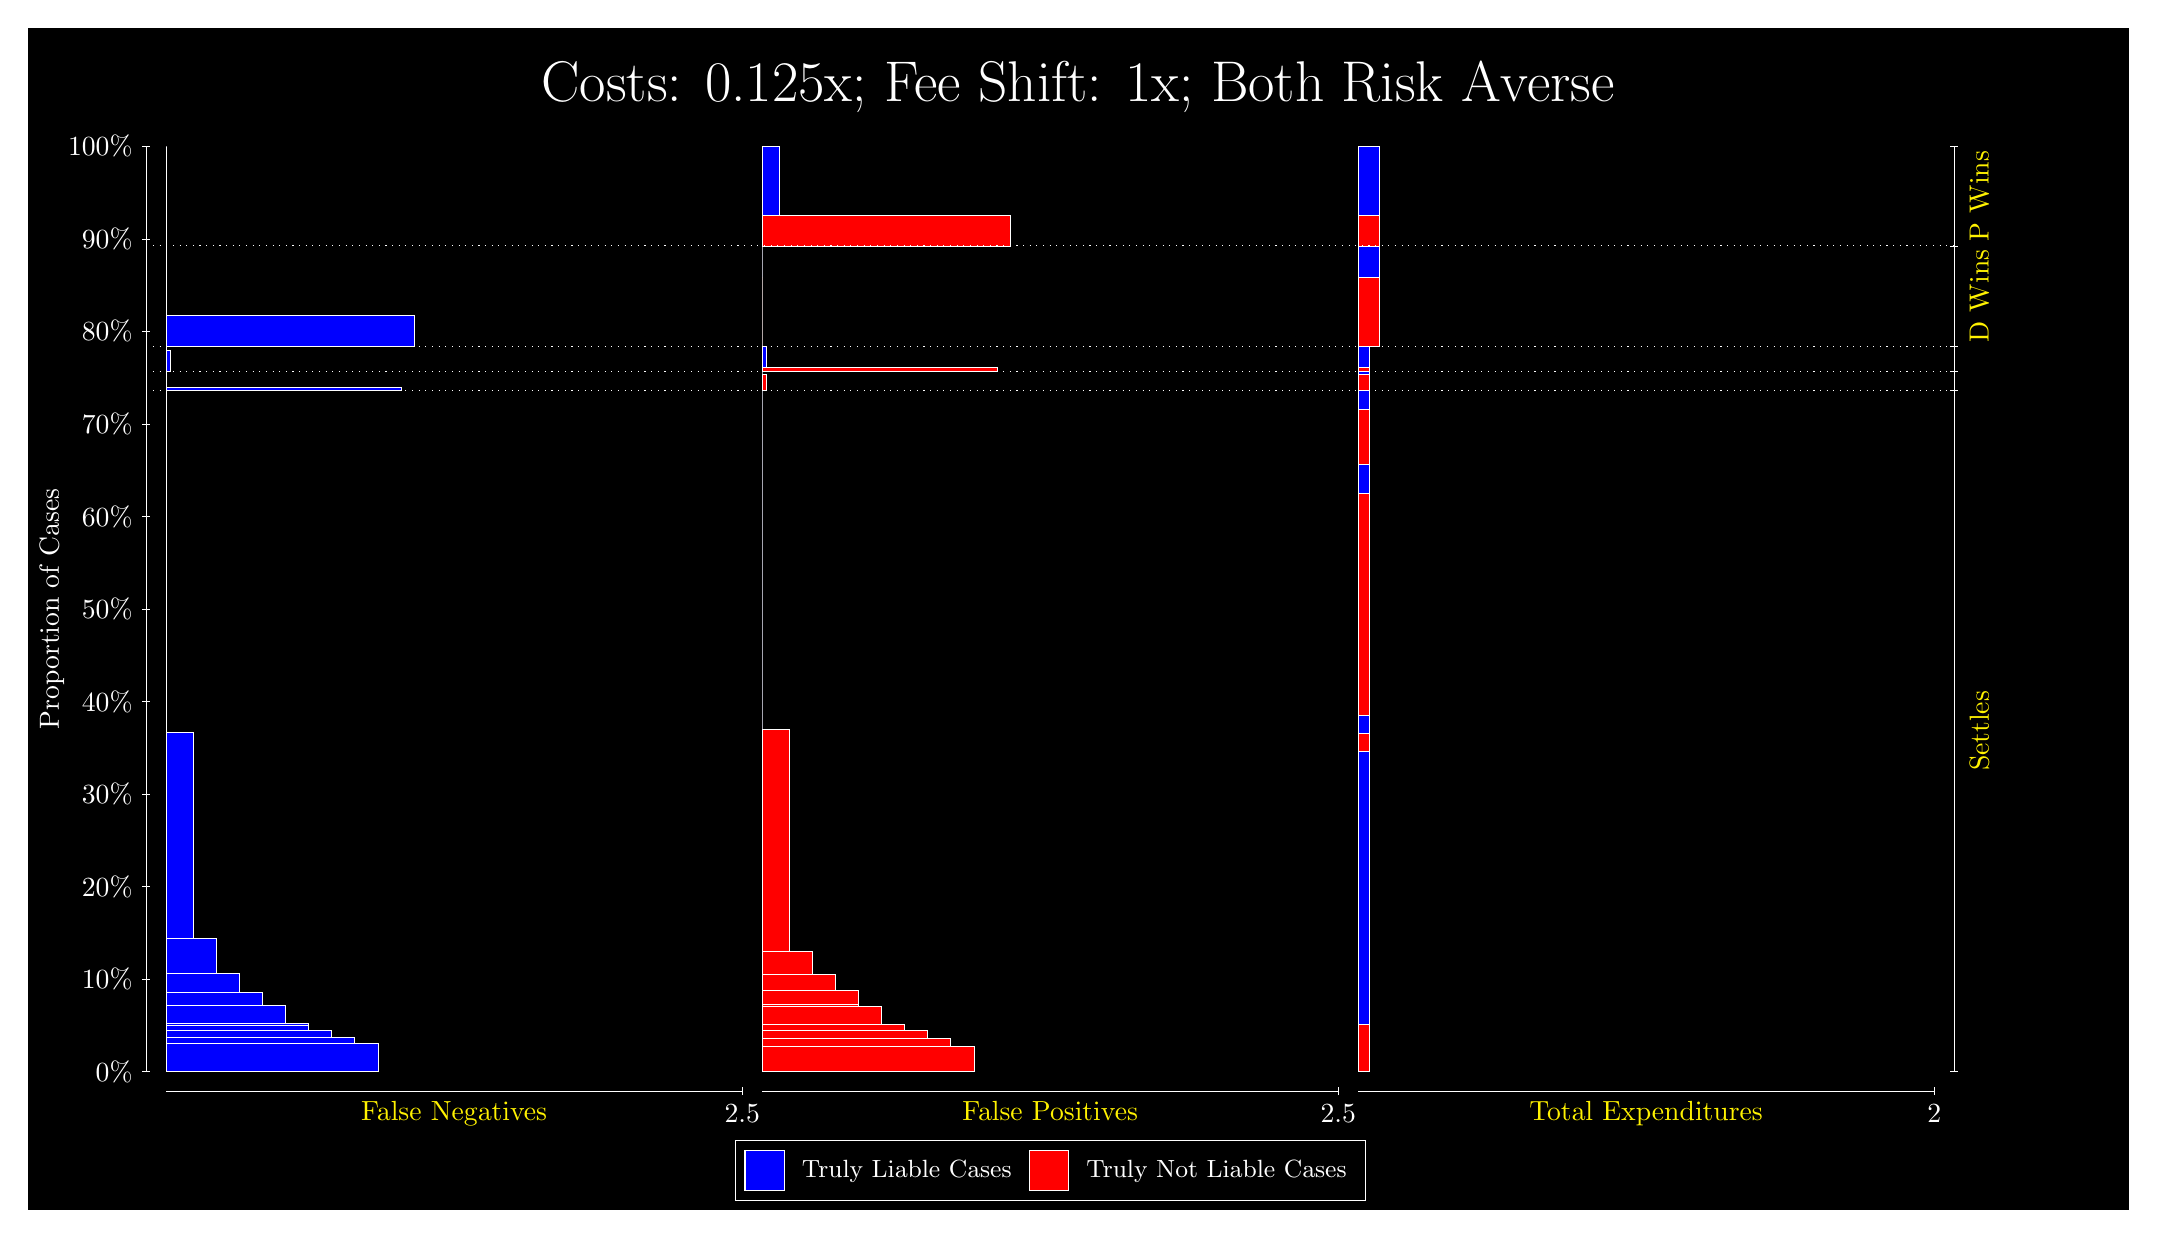
\begin{tikzpicture}
\draw[fill=black] (0,0) rectangle (26.667,15);
\draw[text=white] (0,13.5) rectangle (26.667,15) node[midway] {\huge Costs: 0.125x; Fee Shift: 1x; Both Risk Averse};
\draw[white, very thin] (1.5,1.75) -- (1.5,13.5);
\node[rotate=90, text=white, anchor=center] at (0.3, 7.625) {Proportion of Cases};
\draw[white, very thin] (1.45,1.75) -- (1.55,1.75);
\node[text=white, anchor=east] at (1.45, 1.75) {0\%};
\draw[white, very thin] (1.45,2.925) -- (1.55,2.925);
\node[text=white, anchor=east] at (1.45, 2.925) {10\%};
\draw[white, very thin] (1.45,4.1) -- (1.55,4.1);
\node[text=white, anchor=east] at (1.45, 4.1) {20\%};
\draw[white, very thin] (1.45,5.275) -- (1.55,5.275);
\node[text=white, anchor=east] at (1.45, 5.275) {30\%};
\draw[white, very thin] (1.45,6.45) -- (1.55,6.45);
\node[text=white, anchor=east] at (1.45, 6.45) {40\%};
\draw[white, very thin] (1.45,7.625) -- (1.55,7.625);
\node[text=white, anchor=east] at (1.45, 7.625) {50\%};
\draw[white, very thin] (1.45,8.8) -- (1.55,8.8);
\node[text=white, anchor=east] at (1.45, 8.8) {60\%};
\draw[white, very thin] (1.45,9.975) -- (1.55,9.975);
\node[text=white, anchor=east] at (1.45, 9.975) {70\%};
\draw[white, very thin] (1.45,11.15) -- (1.55,11.15);
\node[text=white, anchor=east] at (1.45, 11.15) {80\%};
\draw[white, very thin] (1.45,12.325) -- (1.55,12.325);
\node[text=white, anchor=east] at (1.45, 12.325) {90\%};
\draw[white, very thin] (1.45,13.5) -- (1.55,13.5);
\node[text=white, anchor=east] at (1.45, 13.5) {100\%};

\draw[white, very thin] (24.457,1.75) -- (24.457,13.5);
\draw[white, very thin] (24.407,1.75) -- (24.507,1.75);
\node[anchor=west] at (24.407, 1.75) {};
\draw[white, very thin] (24.407,10.402) -- (24.507,10.402);
\node[anchor=west] at (24.407, 10.402) {};
\draw[white, very thin] (24.407,10.644) -- (24.507,10.644);
\node[anchor=west] at (24.407, 10.644) {};
\draw[white, very thin] (24.407,10.963) -- (24.507,10.963);
\node[anchor=west] at (24.407, 10.963) {};
\draw[white, very thin] (24.407,12.235) -- (24.507,12.235);
\node[anchor=west] at (24.407, 12.235) {};
\draw[white, very thin] (24.407,13.5) -- (24.507,13.5);
\node[anchor=west] at (24.407, 13.5) {};

\draw[white, very thin, fill=blue] (1.75,1.75) rectangle (4.4397,2.1121);
\draw[white, very thin, fill=blue] (1.75,2.1121) rectangle (4.1469,2.1842);
\draw[white, very thin, fill=blue] (1.75,2.1842) rectangle (3.8542,2.2692);
\draw[white, very thin, fill=blue] (1.75,2.2692) rectangle (3.5614,2.3336);
\draw[white, very thin, fill=blue] (1.75,2.3336) rectangle (3.5614,2.358);
\draw[white, very thin, fill=blue] (1.75,2.358) rectangle (3.2687,2.5875);
\draw[white, very thin, fill=blue] (1.75,2.5875) rectangle (2.9759,2.7571);
\draw[white, very thin, fill=blue] (1.75,2.7571) rectangle (2.6832,2.9948);
\draw[white, very thin, fill=blue] (1.75,2.9948) rectangle (2.3904,3.4456);
\draw[white, very thin, fill=blue] (1.75,3.4456) rectangle (2.0976,6.053);
\draw[white, very thin, fill=red] (1.75,6.053) rectangle (1.75,10.402);
\draw[white, very thin, fill=blue] (1.75,10.402) rectangle (4.7324,10.442);
\draw[white, very thin, fill=red] (1.75,10.442) rectangle (1.75,10.644);
\draw[white, very thin, fill=blue] (1.75,10.644) rectangle (1.8049,10.911);
\draw[white, very thin, fill=red] (1.75,10.911) rectangle (1.75,10.963);
\draw[white, very thin, fill=blue] (1.75,10.963) rectangle (4.8971,11.358);
\draw[white, very thin, fill=red] (1.75,11.358) rectangle (1.75,12.235);
\draw[white, very thin, fill=red] (1.75,12.235) rectangle (1.75,12.63);
\draw[white, very thin, fill=blue] (1.75,12.63) rectangle (1.75,13.5);
\draw[white, very thin, fill=red] (9.3189,1.75) rectangle (12.009,2.0732);
\draw[white, very thin, fill=red] (9.3189,2.0732) rectangle (11.716,2.1733);
\draw[white, very thin, fill=red] (9.3189,2.1733) rectangle (11.423,2.2741);
\draw[white, very thin, fill=red] (9.3189,2.2741) rectangle (11.13,2.3548);
\draw[white, very thin, fill=red] (9.3189,2.3548) rectangle (10.838,2.5818);
\draw[white, very thin, fill=red] (9.3189,2.5818) rectangle (10.545,2.6079);
\draw[white, very thin, fill=red] (9.3189,2.6079) rectangle (10.545,2.7769);
\draw[white, very thin, fill=red] (9.3189,2.7769) rectangle (10.252,2.9812);
\draw[white, very thin, fill=red] (9.3189,2.9812) rectangle (9.9593,3.278);
\draw[white, very thin, fill=red] (9.3189,3.278) rectangle (9.6665,6.0995);
\draw[white, very thin, fill=blue] (9.3189,6.0995) rectangle (9.3189,10.402);
\draw[white, very thin, fill=red] (9.3189,10.402) rectangle (9.3738,10.604);
\draw[white, very thin, fill=blue] (9.3189,10.604) rectangle (9.3189,10.644);
\draw[white, very thin, fill=red] (9.3189,10.644) rectangle (12.301,10.696);
\draw[white, very thin, fill=blue] (9.3189,10.696) rectangle (9.3738,10.963);
\draw[white, very thin, fill=red] (9.3189,10.963) rectangle (9.3189,11.839);
\draw[white, very thin, fill=blue] (9.3189,11.839) rectangle (9.3189,12.235);
\draw[white, very thin, fill=red] (9.3189,12.235) rectangle (12.466,12.63);
\draw[white, very thin, fill=blue] (9.3189,12.63) rectangle (9.5384,13.5);
\draw[white, very thin, fill=red] (16.888,1.75) rectangle (17.025,2.3548);
\draw[white, very thin, fill=blue] (16.888,2.3548) rectangle (17.025,5.8203);
\draw[white, very thin, fill=red] (16.888,5.8203) rectangle (17.025,6.0472);
\draw[white, very thin, fill=blue] (16.888,6.0472) rectangle (17.025,6.2768);
\draw[white, very thin, fill=red] (16.888,6.2768) rectangle (17.025,9.0982);
\draw[white, very thin, fill=blue] (16.888,9.0982) rectangle (17.025,9.4603);
\draw[white, very thin, fill=red] (16.888,9.4603) rectangle (17.025,10.157);
\draw[white, very thin, fill=blue] (16.888,10.157) rectangle (17.025,10.402);
\draw[white, very thin, fill=red] (16.888,10.402) rectangle (17.025,10.604);
\draw[white, very thin, fill=blue] (16.888,10.604) rectangle (17.025,10.644);
\draw[white, very thin, fill=red] (16.888,10.644) rectangle (17.025,10.696);
\draw[white, very thin, fill=blue] (16.888,10.696) rectangle (17.025,10.963);
\draw[white, very thin, fill=red] (16.888,10.963) rectangle (17.162,11.839);
\draw[white, very thin, fill=blue] (16.888,11.839) rectangle (17.162,12.235);
\draw[white, very thin, fill=red] (16.888,12.235) rectangle (17.162,12.63);
\draw[white, very thin, fill=blue] (16.888,12.63) rectangle (17.162,13.5);
\draw[white, dotted] (1.5,10.402) -- (24.457,10.402);
\draw[white, dotted] (1.5,10.644) -- (24.457,10.644);
\draw[white, dotted] (1.5,10.963) -- (24.457,10.963);
\draw[white, dotted] (1.5,12.235) -- (24.457,12.235);
\draw[white, very thin] (1.75,1.5) -- (9.0689,1.5);
\node[text=yellow, anchor=north] at (5.4094, 1.5) {False Negatives};
\draw[white, very thin] (9.0689,1.45) -- (9.0689,1.55);
\node[text=white, anchor=north] at (9.0689, 1.45) {2.5};

\draw[white, very thin] (9.3189,1.5) -- (16.638,1.5);
\node[text=yellow, anchor=north] at (12.978, 1.5) {False Positives};
\draw[white, very thin] (16.638,1.45) -- (16.638,1.55);
\node[text=white, anchor=north] at (16.638, 1.45) {2.5};

\draw[white, very thin] (16.888,1.5) -- (24.207,1.5);
\node[text=yellow, anchor=north] at (20.547, 1.5) {Total Expenditures};
\draw[white, very thin] (24.207,1.45) -- (24.207,1.55);
\node[text=white, anchor=north] at (24.207, 1.45) {2};

\node[text=yellow, centered, rotate=90] at (24.777, 6.0762) {Settles};


\node[text=yellow, centered, rotate=90] at (24.777, 11.599) {D Wins};
\node[text=yellow, centered, rotate=90] at (24.777, 12.867) {P Wins};

\draw (12.978300999999998,1.5) node[draw=none] (baseCoordinate) {};
\begin{scope}[align=center]
        \matrix[scale=0.5, draw=white, below=0.5cm of baseCoordinate, nodes={draw}, column sep=0.1cm]{
            \node[rectangle, draw, minimum width=0.5cm, minimum height=0.5cm, fill=blue] {}; &
            \node[draw=none, font=\small, text=white] (B) {Truly Liable Cases}; &
            \node[rectangle, draw, minimum width=0.5cm, minimum height=0.5cm, fill=red] {}; &
            \node[draw=none, font=\small, text=white] (B) {Truly Not Liable Cases}; \\
            };
\end{scope}

\end{tikzpicture}
\end{document}